% Metodología: predictores, modelos, origen móvil y evaluación.
% Protocolo de notebooks/02_modelado.ipynb (secciones 6 a 12).
\documentclass[border=2pt]{standalone}
% Estilo común de los diagramas: letra sin serifa, como las figuras del
% notebook, y ancho máximo de una columna IEEE (8,9 cm). Compilar con pdflatex.
\usepackage[utf8]{inputenc}
\usepackage[T1]{fontenc}
\usepackage{tgheros}
\renewcommand{\familydefault}{\sfdefault}
\usepackage{tikz}
\usetikzlibrary{positioning, arrows.meta, fit, backgrounds, calc}

\definecolor{pm}{HTML}{1F77B4}
\definecolor{meteo}{HTML}{2CA02C}
\definecolor{modelo}{HTML}{FF7F0E}
\definecolor{perdida}{HTML}{B22222}
\definecolor{gris}{HTML}{6E6E6E}

\tikzset{
  caja/.style={draw=#1, fill=#1!8, rounded corners=2pt, line width=0.6pt,
    align=center, inner sep=3pt, font=\fontsize{6.5}{7.8}\selectfont},
  caja/.default=gris,
  flecha/.style={-{Stealth[length=4pt]}, line width=0.6pt, draw=gris},
  nota/.style={font=\fontsize{5.8}{7}\selectfont, text=perdida, align=left},
  titulo/.style={font=\fontsize{6.5}{7.8}\selectfont\bfseries, text=#1},
}
\newcommand{\menos}[1]{\textcolor{perdida}{\fontsize{5.8}{7}\selectfont #1}}


\begin{document}
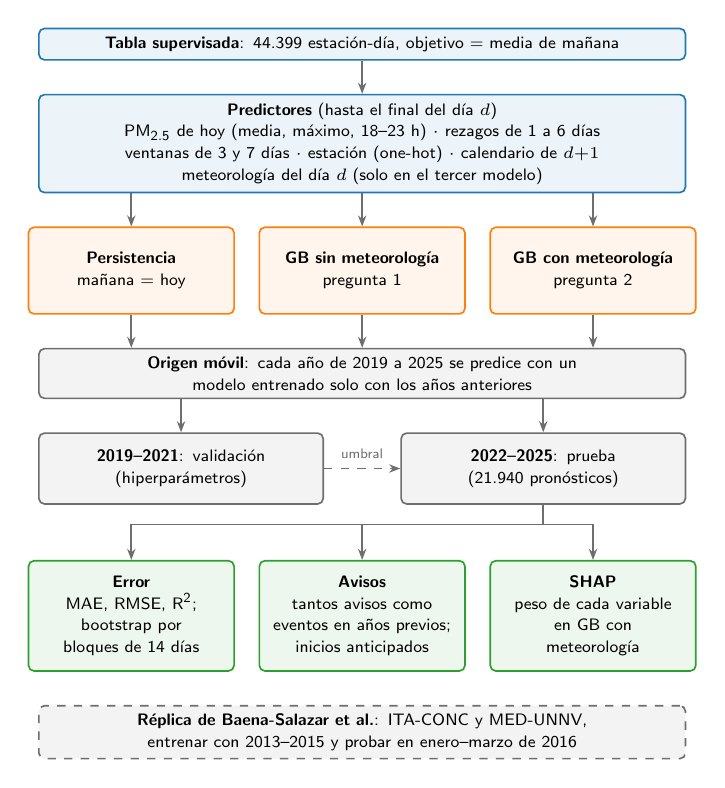
\begin{tikzpicture}[node distance=4.2mm]
  \node[caja=pm, text width=80mm] (tabla)
    {\textbf{Tabla supervisada}: 44.399 estación-día, objetivo = media de mañana};
  \node[caja=pm, text width=80mm, below=of tabla] (pred)
    {\textbf{Predictores} (hasta el final del día $d$)\\
     PM\textsubscript{2.5} de hoy (media, máximo, 18--23 h) $\cdot$ rezagos de 1 a 6 días\\
     ventanas de 3 y 7 días $\cdot$ estación (one-hot) $\cdot$ calendario de $d{+}1$\\
     meteorología del día $d$ (solo en el tercer modelo)};

  \node[caja=modelo, text width=24mm, minimum height=11mm, below=of pred] (gbs)
    {\textbf{GB sin meteorología}\\pregunta 1};
  \node[caja=modelo, text width=24mm, minimum height=11mm, left=3mm of gbs] (pers)
    {\textbf{Persistencia}\\mañana = hoy};
  \node[caja=modelo, text width=24mm, minimum height=11mm, right=3mm of gbs] (gbc)
    {\textbf{GB con meteorología}\\pregunta 2};

  \node[caja, text width=80mm, below=of gbs] (om)
    {\textbf{Origen móvil}: cada año de 2019 a 2025 se predice con un\\
     modelo entrenado solo con los años anteriores};
  \node[caja, text width=34mm, minimum height=9mm, below=of om.south west, anchor=north west] (cal)
    {\textbf{2019--2021}: validación\\(hiperparámetros)};
  \node[caja, text width=34mm, minimum height=9mm, below=of om.south east, anchor=north east] (prueba)
    {\textbf{2022--2025}: prueba\\(21.940 pronósticos)};

  \node[caja=meteo, text width=24mm, minimum height=14mm, below=7mm of prueba.south -| gbs] (aviso)
    {\textbf{Avisos}\\tantos avisos como\\eventos en años previos;\\inicios anticipados};
  \node[caja=meteo, text width=24mm, minimum height=14mm, left=3mm of aviso] (error)
    {\textbf{Error}\\MAE, RMSE, R\textsuperscript{2};\\bootstrap por\\bloques de 14 días};
  \node[caja=meteo, text width=24mm, minimum height=14mm, right=3mm of aviso] (shap)
    {\textbf{SHAP}\\peso de cada variable\\en GB con\\meteorología};

  \node[caja, dashed, text width=80mm, below=of aviso] (baena)
    {\textbf{Réplica de Baena-Salazar et al.}: ITA-CONC y MED-UNNV,\\
     entrenar con 2013--2015 y probar en enero--marzo de 2016};

  \draw[flecha] (tabla) -- (pred);
  \foreach \m in {pers, gbs, gbc} \draw[flecha] (pred.south -| \m) -- (\m);
  \foreach \m in {pers, gbs, gbc} \draw[flecha] (\m) -- (om.north -| \m);
  \draw[flecha] (cal.north |- om.south) -- (cal);
  \draw[flecha] (prueba.north |- om.south) -- (prueba);
  \draw[flecha, dashed] (cal.east) -- (prueba.west) node[midway, above, font=\fontsize{5.5}{6}\selectfont, text=gris] {umbral};
  \foreach \m in {error, aviso, shap} \draw[flecha] (prueba.south) -- ++(0,-2.5mm) -| (\m.north);
\end{tikzpicture}
\end{document}
